

\section*{K4/1. feladat: Fojtószelepes ammónia hűtőgép}
\addcontentsline{toc}{section}{K4/1. feladat: Hőterjedés sík kazánfalban}

\begin{tabular}{ | p{2cm} | p{14cm} | } 
	\hline
	Név & Steiber Árpád \\ 
	\hline
	Szak & Vegyészmérnöki \\ 
	\hline
	Félév & 2019/2020 II. (tavaszi) félév \\ 
	\hline
\end{tabular}
\vspace{0.5cm}

\noindent Kiszámítandó a három rétegű végtelennek tekinthető sík fal \SI{6}{\meter\squared} felületen átadódó hőáram, stacionárius, hőforrás nélküli esetben, ha az adatok a következők:
\begin{center}
	$\delta_1 = \SI{10}{\milli\meter}$ $\lambda_1 = \SI{0.1}{\watt\per\meter\kelvin}$ \\
	\vspace{2mm}
	$\delta_2 = \SI{20}{\milli\meter}$ $\lambda_1 = \SI{0.15}{\watt\per\meter\kelvin}$ \\
	\vspace{2mm}
	$\delta_2 = \SI{30}{\milli\meter}$ $\lambda_1 = \SI{0.03}{\watt\per\meter\kelvin}$ \\
\end{center}

\vspace{2mm}

A fal külső felületein a hőmérséklet $T_1 = \SI{500}{\celsius}$ és $T_4 = \SI{65}{\celsius}$. Mennyi az érintkező felületek hőmérséklete? Rajzolja fel a hőmérséklet-hely függvényt!

\vspace{2mm}

\begin{figure}[h]
	\centering
	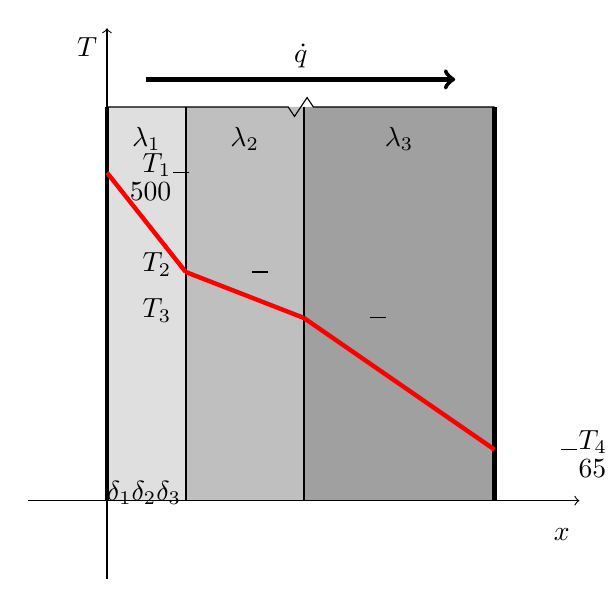
\begin{tikzpicture}
	\pgfmathsetmacro{\d}{32/6.5}
	\pgfmathsetmacro{\L}{5}
	\pgfmathsetmacro{\TA}{500/120}
	\pgfmathsetmacro{\TC}{464.7/160}
	\pgfmathsetmacro{\TD}{417.8/180}
	\pgfmathsetmacro{\TB}{65/100}
	\pgfmathsetmacro{\TK}{(\TA+\TB)/2}
	
	% Fal
	\fill[gray,opacity=0.25] (0,0) -- (1,0) -- (1, \L) -- (0, \L) -- (0,0);
	\fill[gray, opacity=0.5] (1,0) -- (2.5,0) -- (2.5, \L) -- (1, \L) -- (1,0);
	\fill[gray, opacity=0.75] (2.5,0) -- (5-0.08,0) -- (5-0.08, \L) -- (2.5, \L) -- (2.5,0);
	\draw[] (0,\L) -- ({\d/2-0.16},\L) -- ({\d/2-0.08}, {\L-0.12}) -- ({\d/2+0.08}, {\L+0.12}) -- ({\d/2+0.16}, \L) -- (\d, \L);
	\draw[ultra thick] (0,0) -- (0,\L);
	\draw[ultra thick] (\d, 0) -- (\d, \L);
	\draw[thick] (1,0) -- (1,\L);
	\draw[thick] (2.5,0) -- (2.5,\L);
	
	% Tengelyek
	\draw[->] (0,-1) -- (0,\L+1) node[anchor=north east]{$T$};
	\draw[->] (-1,0) -- (6,0) node[anchor=base east, shift={(0,-0.5)}]{$x$};
	
	% Hőáram és hőáramsűrűség
	\draw[->, ultra thick] (0.5,{\L+0.35}) -- ({\d/2},{\L+0.35}) node[anchor=south]{$\dot{q}$} -- ({\d - 0.5},{\L+0.35});
	
	% A hővezetési tényező
	\node[anchor=base] at ({0.5},{\L-0.5}) {$\lambda_1$};
	\node[anchor=base] at ({1.75},{\L-0.5}) {$\lambda_2$};
	\node[anchor=base] at ({3.71},{\L-0.5}) {$\lambda_3$};
	
	% T(x)
	\draw[red, ultra thick] (0,\TA) -- (1,\TC);
	\draw[red, ultra thick] (1,\TC) -- (2.5,\TD);
	\draw[red, ultra thick] (2.5,\TD) -- (5-0.08,\TB);
	% A delta falvastagságok
	\pgflength[xa=0, ya=0, xb=1-0.001, yb=0, alim=0]{$\delta_1$};
	\pgflength[xa=1-0.001, ya=0, xb=2.5, yb=0, alim=0]{$\delta_2$};
	\pgflength[xa=2.5, ya=0, xb=5-0.08, yb=0, alim=0]{$\delta_3$};
	
	% A hőmérséklet értékek
	\draw (-0.1,\TA) -- (0.1,\TA);
	\node[anchor=base east] at (0,\TA) {$T_1$};
	\node[anchor=north east] at (0,\TA) {$\SI{500}{\celsius}$};
	
	\draw (0.9,\TC) -- (1.1,\TC);
	\node[anchor=base east] at (0,\TC) {$T_2$};
	
	\draw (2.4,\TD) -- (2.6,\TD);
	\node[anchor=base east] at (0,\TD) {$T_3$};
	
	\draw (-0.1+\d,\TB) -- (0.1+\d,\TB);
	\node[anchor=base west] at (\d,\TB) {$T_4$};
	\node[anchor=north west] at (\d,\TB) {$\SI{65}{\celsius}$};
	
	
	\end{tikzpicture}
	\caption{A hőmérséklet-hely függvény}
\end{figure}



FOURIER törvénye szerint egy homogén testben a hőáram a csökkenő
hőmérsékletek irányába mutat, arányos a terjedési irányú, hosszegységenkénti
hőmérséklet-változással és az erre az irányra merőleges keresztmetszettel. 
\begin{equation}
\dot{Q} = \lambda F \frac{dT}{dx} 
\end{equation}

A hőáram és a keresztmetszet hányadosa a hőáramsűrűség.
\begin{equation}
\dot{q} = \frac{\dot{Q}}{F}
\end{equation}
A dT/dx hányados a hőmérséklet különbség és a fal vastagságának hányadosa.
A hőáramsűrűség tehát:
\begin{equation}
\dot{q} = \frac{\lambda}{\delta} (T_1 - T_2) 
\end{equation}


Mivel a hőáramsűrűség állandó, ezért az 5.26 egyenletet ha felírjuk az összes falra, akkor az alábbi egyenletet kapjuk.
\begin{equation}
\dot{q} = \frac{\lambda_1}{\delta_1} (T_1 - T_2) = \frac{\lambda_2}{\delta_2} (T_2 - T_3) = \frac{\lambda_3}{\delta_3} (T_3 - T_4)
\end{equation}

Egy kis átalakítással az alábbi általános képlethez jutunk.
\begin{equation}
\dot{q} = \frac{1}{\underset{i=1}{\overset{n}{\Sigma}}\frac{\delta_n}{\lambda_n}} \Delta T
\end{equation}
A jobb oldalon szereplő első tag a hőátszármaztatási tényező($\kappa$). A feladat megoldásának első lépéseként ezt a tényezőt kell meghatároznunk.
\begin{equation}
\kappa = \frac{1}{\frac{\delta_1}{\lambda_1}+\frac{\delta_2}{\lambda_2}+\frac{\delta_3}{\lambda_3}} = \frac{1}{\frac{\SI{0.01}{\meter}}{\SI{0.1}{\watt\per\meter\kelvin}} + \frac{\SI{0.02}{\meter}}{\SI{0.15}{\watt\per\meter\kelvin}} +
	\frac{\SI{0.03}{\meter}}{\SI{0.03}{\watt\per\meter\kelvin}}} = \SI{0.811}{\watt\per\meter\squared\kelvin}
\end{equation}


Az 5.28. egyenlet segítségével már könnyen meghatározható a hőáramsűrűség.
\begin{equation}
\dot{q} =  \frac{1}{\frac{\delta_1}{\lambda_1}+\frac{\delta_2}{\lambda_2}+\frac{\delta_3}{\lambda_3}} (T_1 - T_4)= \frac{1}{\frac{\SI{0.01}{\meter}}{\SI{0.1}{\watt\per\meter\kelvin}} + \frac{\SI{0.02}{\meter}}{\SI{0.15}{\watt\per\meter\kelvin}} +
	\frac{\SI{0.03}{\meter}}{\SI{0.03}{\watt\per\meter\kelvin}}} (\SI{500}{\celsius} - \SI{65}{\celsius}) \\
= \SI{352.70}{\watt\per\meter\squared}
\end{equation}

Az 5.25. egyenlet alapján a hőáram 
\begin{equation}
\dot{Q} = \dot{q} F = \SI{352.70}{\watt\per\meter\squared} \SI{6}{\meter\squared} = \SI{2116.2}{\watt}
\end{equation}

Az érintkező felületek kiszámítása az 5.27. egyenlet alapján
\begin{equation}
\SI{352.7}{\watt\per\meter\squared} = \frac{\SI{0.1}{\watt\per\meter\kelvin}}{\SI{0.01}{\meter}} (\SI{500}{\celsius} - T_2) 
\end{equation}
\begin{center}
	$T_2$ = \SI{464.72}{\celsius}
\end{center}

\begin{equation}
\SI{352.7}{\watt\per\meter\squared} = \frac{\SI{0.15}{\watt\per\meter\kelvin}}{\SI{0.02}{\meter}} (\SI{464,72}{\celsius} - T_3) 
\end{equation}
\begin{center}
	$T_3$ = \SI{417.80}{\celsius}
\end{center}

\pagebreak


\end{equation}

\begin{equation}
	T_1' = T_2' + \frac{\delta_1}{\lambda_1}\dot{q}_a = \SI{593}{\celsius} + \frac{\SI{16}{\milli\meter}}{\SI{43}{\watt\per\meter\kelvin}} \SI{524}{\kilo\watt\per\meter\squared} = \SI{788}{\celsius}
\end{equation}

\subsubsection*{c) Ha szilárdsági okok miatt a fal hőmérséklete nem emelkedhet, de a gőznyomás változatlan, mekkora lesz a hőáramsűrűség?}